\documentclass[11pt,a4paper]{article}

\usepackage[utf8]{inputenc}
\usepackage[margin=1in]{geometry}
\usepackage{graphicx}
\usepackage{booktabs}
\usepackage{listings}
\usepackage{xcolor}
\usepackage{float}
\usepackage{parskip}

\definecolor{codegreen}{rgb}{0,0.6,0}
\definecolor{codegray}{rgb}{0.5,0.5,0.5}
\definecolor{backcolour}{rgb}{0.95,0.95,0.92}

\lstdefinestyle{pythonstyle}{
    backgroundcolor=\color{backcolour},
    commentstyle=\color{codegreen},
    keywordstyle=\color{blue},
    numberstyle=\tiny\color{codegray},
    basicstyle=\ttfamily\footnotesize,
    breaklines=true,
    numbers=left,
    numbersep=5pt,
    language=Python
}
\lstset{style=pythonstyle}

\title{Assignment 1: LLM Code Generation Evaluation\\
\large Fibonacci Sequence Generation with a Small Language Model}
\author{
    Student ID: 12349031 \\
    \small Course: 700.390 Advanced Topics in Neurocomputing:\\
    \small Explainability, Neuro-Symbolic Computing, AI Agents, LLM,\\
    \small Quantum Computing, PINN
}
\date{July 1, 2026}

\begin{document}

\maketitle

\section{Introduction}

This assignment evaluates how well a small language model can generate correct Python code for a simple algorithmic task. The task is to generate programs that compute and print all Fibonacci numbers less than 100. Two types of implementations were tested: iterative and recursive. The main focus was on how the temperature parameter affects the quality of the generated code.

\section{Methodology}

\subsection{Model}

The model used is \textbf{Qwen/Qwen2.5-Coder-0.5B-Instruct} \cite{qwen2025coder}, a 0.5 billion parameter instruction-tuned model built for code generation. It was chosen because it is small enough to run without heavy hardware but still capable of following coding instructions.

\subsection{Setup}

The model was run on Google Colab using an A100 GPU. For each experiment, the model received a prompt asking it to write a Python program implementing the Fibonacci sequence (either iterative or recursive) and print all values less than 100.

The expected correct output is: \texttt{0, 1, 1, 2, 3, 5, 8, 13, 21, 34, 55, 89}

\subsection{Tested Settings}

\begin{table}[H]
\centering
\caption{Experiment Configuration}
\begin{tabular}{ll}
\toprule
\textbf{Parameter} & \textbf{Values} \\
\midrule
Temperature & 0.0, 0.3, 0.5, 0.7 \\
Top-p & 0.95 \\
Top-k & 50 \\
Trials per config & 2 \\
Implementation types & Iterative, Recursive \\
Total experiments & 16 \\
\bottomrule
\end{tabular}
\end{table}

Temperature controls how random the model's token selection is. At 0.0 the model always picks the most likely next token (greedy). Higher values introduce more randomness. Top-p and top-k limit which tokens are considered during sampling.

Each generated program was automatically executed and its output was compared to the expected Fibonacci sequence. Three things were checked: whether the code ran without errors (executability), whether the output contained the right numbers (correctness), and whether it was an exact match.

\section{Results and Observations}

\subsection{Overall Results}

\begin{table}[H]
\centering
\caption{Overall Performance Across All 16 Experiments}
\begin{tabular}{lccc}
\toprule
\textbf{Metric} & \textbf{Overall} & \textbf{Iterative} & \textbf{Recursive} \\
\midrule
Executable  & 100\% & 100\% & 100\% \\
Correct     & 25\%  & 50\%  & 0\%   \\
Exact Match & 25\%  & 50\%  & 0\%   \\
\bottomrule
\end{tabular}
\end{table}

\subsection{Effect of Temperature}

\begin{table}[H]
\centering
\caption{Correctness Rate by Temperature (both implementation types combined)}
\begin{tabular}{lcc}
\toprule
\textbf{Temperature} & \textbf{Correct / Total} & \textbf{Correctness Rate} \\
\midrule
0.0 & 0 / 4 & 0\%  \\
0.3 & 1 / 4 & 25\% \\
0.5 & 1 / 4 & 25\% \\
0.7 & 2 / 4 & 50\% \\
\bottomrule
\end{tabular}
\end{table}

\begin{figure}[H]
\centering
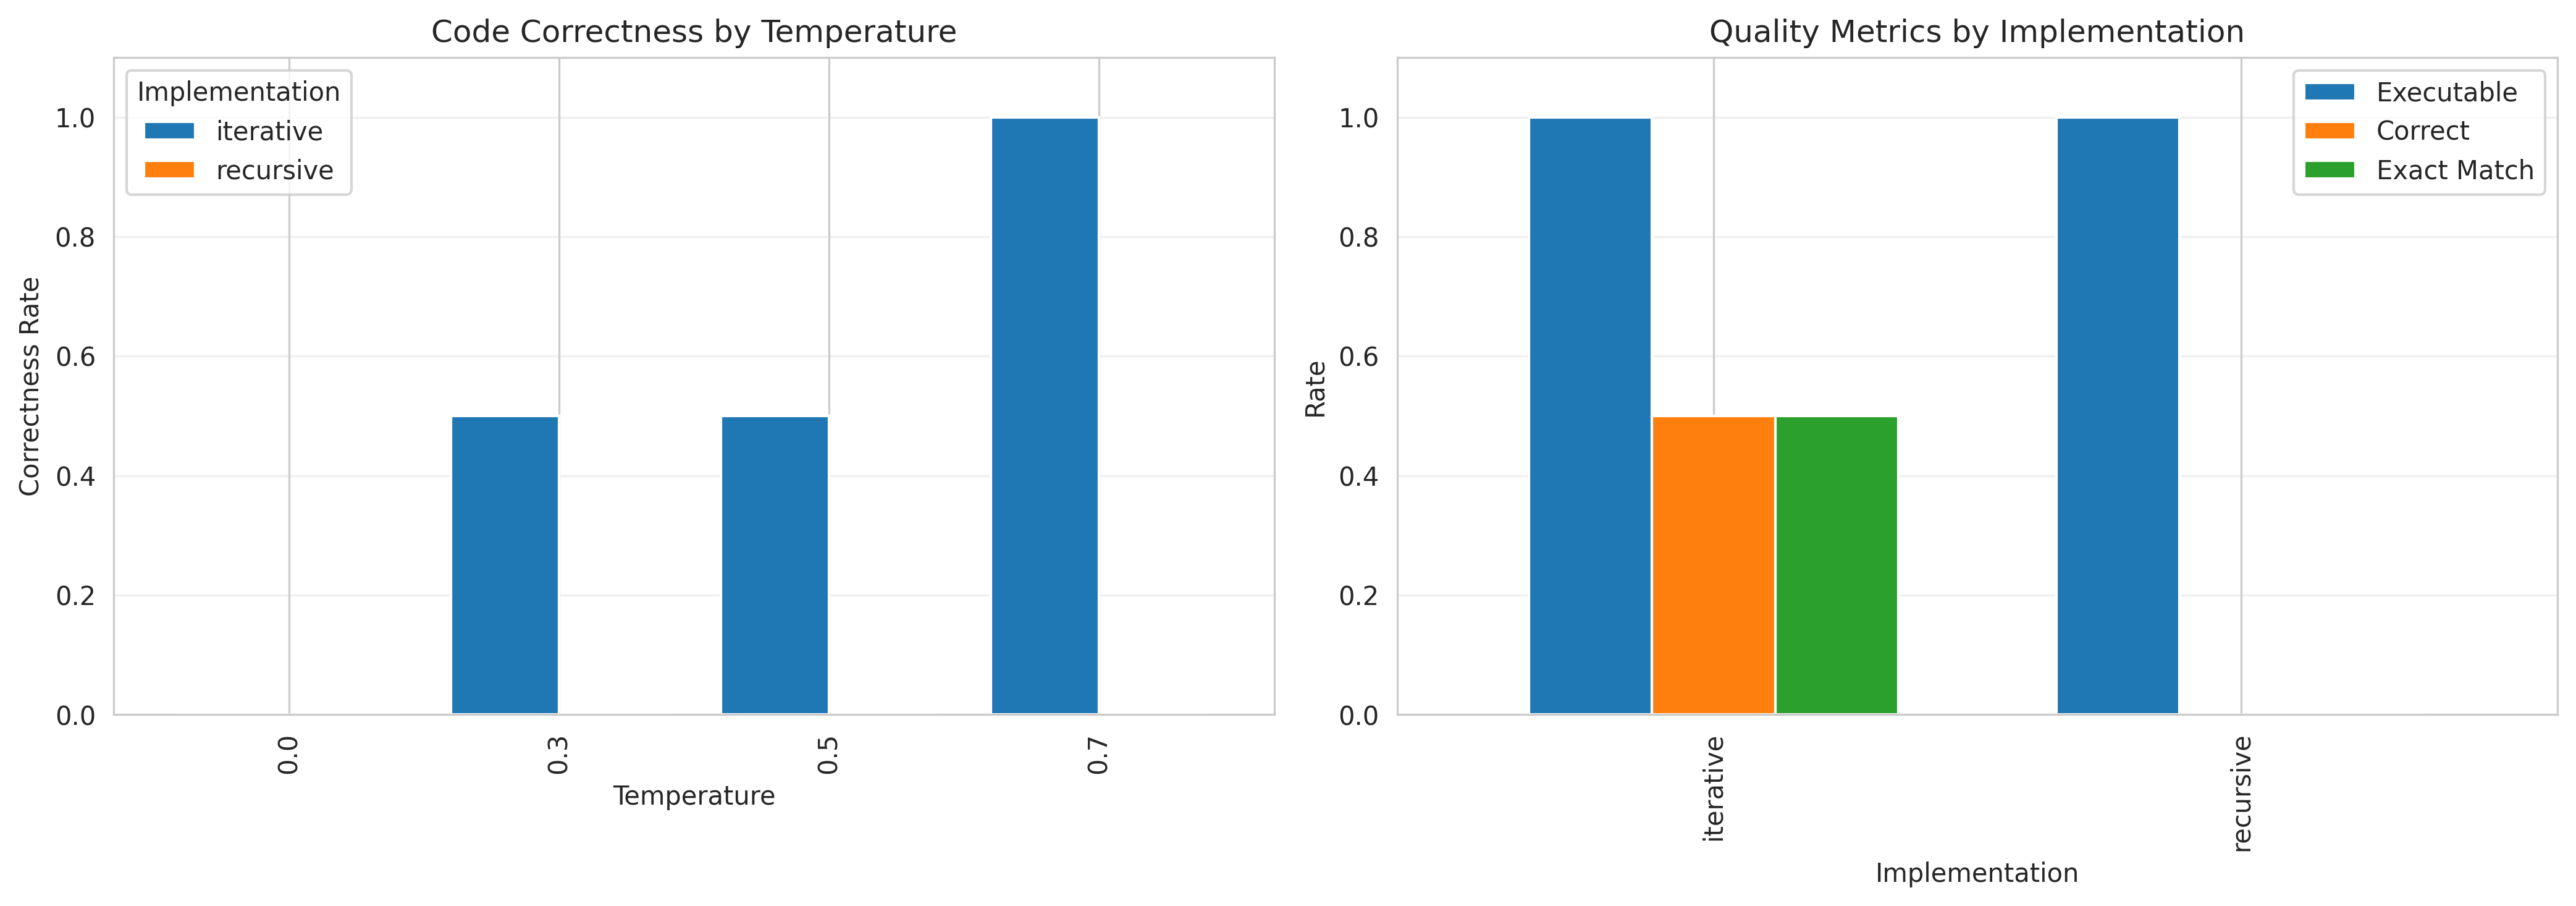
\includegraphics[width=0.9\textwidth]{figures/analysis_overview.png}
\caption{Left: Correctness by temperature for each implementation type. Right: Overall quality metrics per implementation.}
\end{figure}

\begin{figure}[H]
\centering
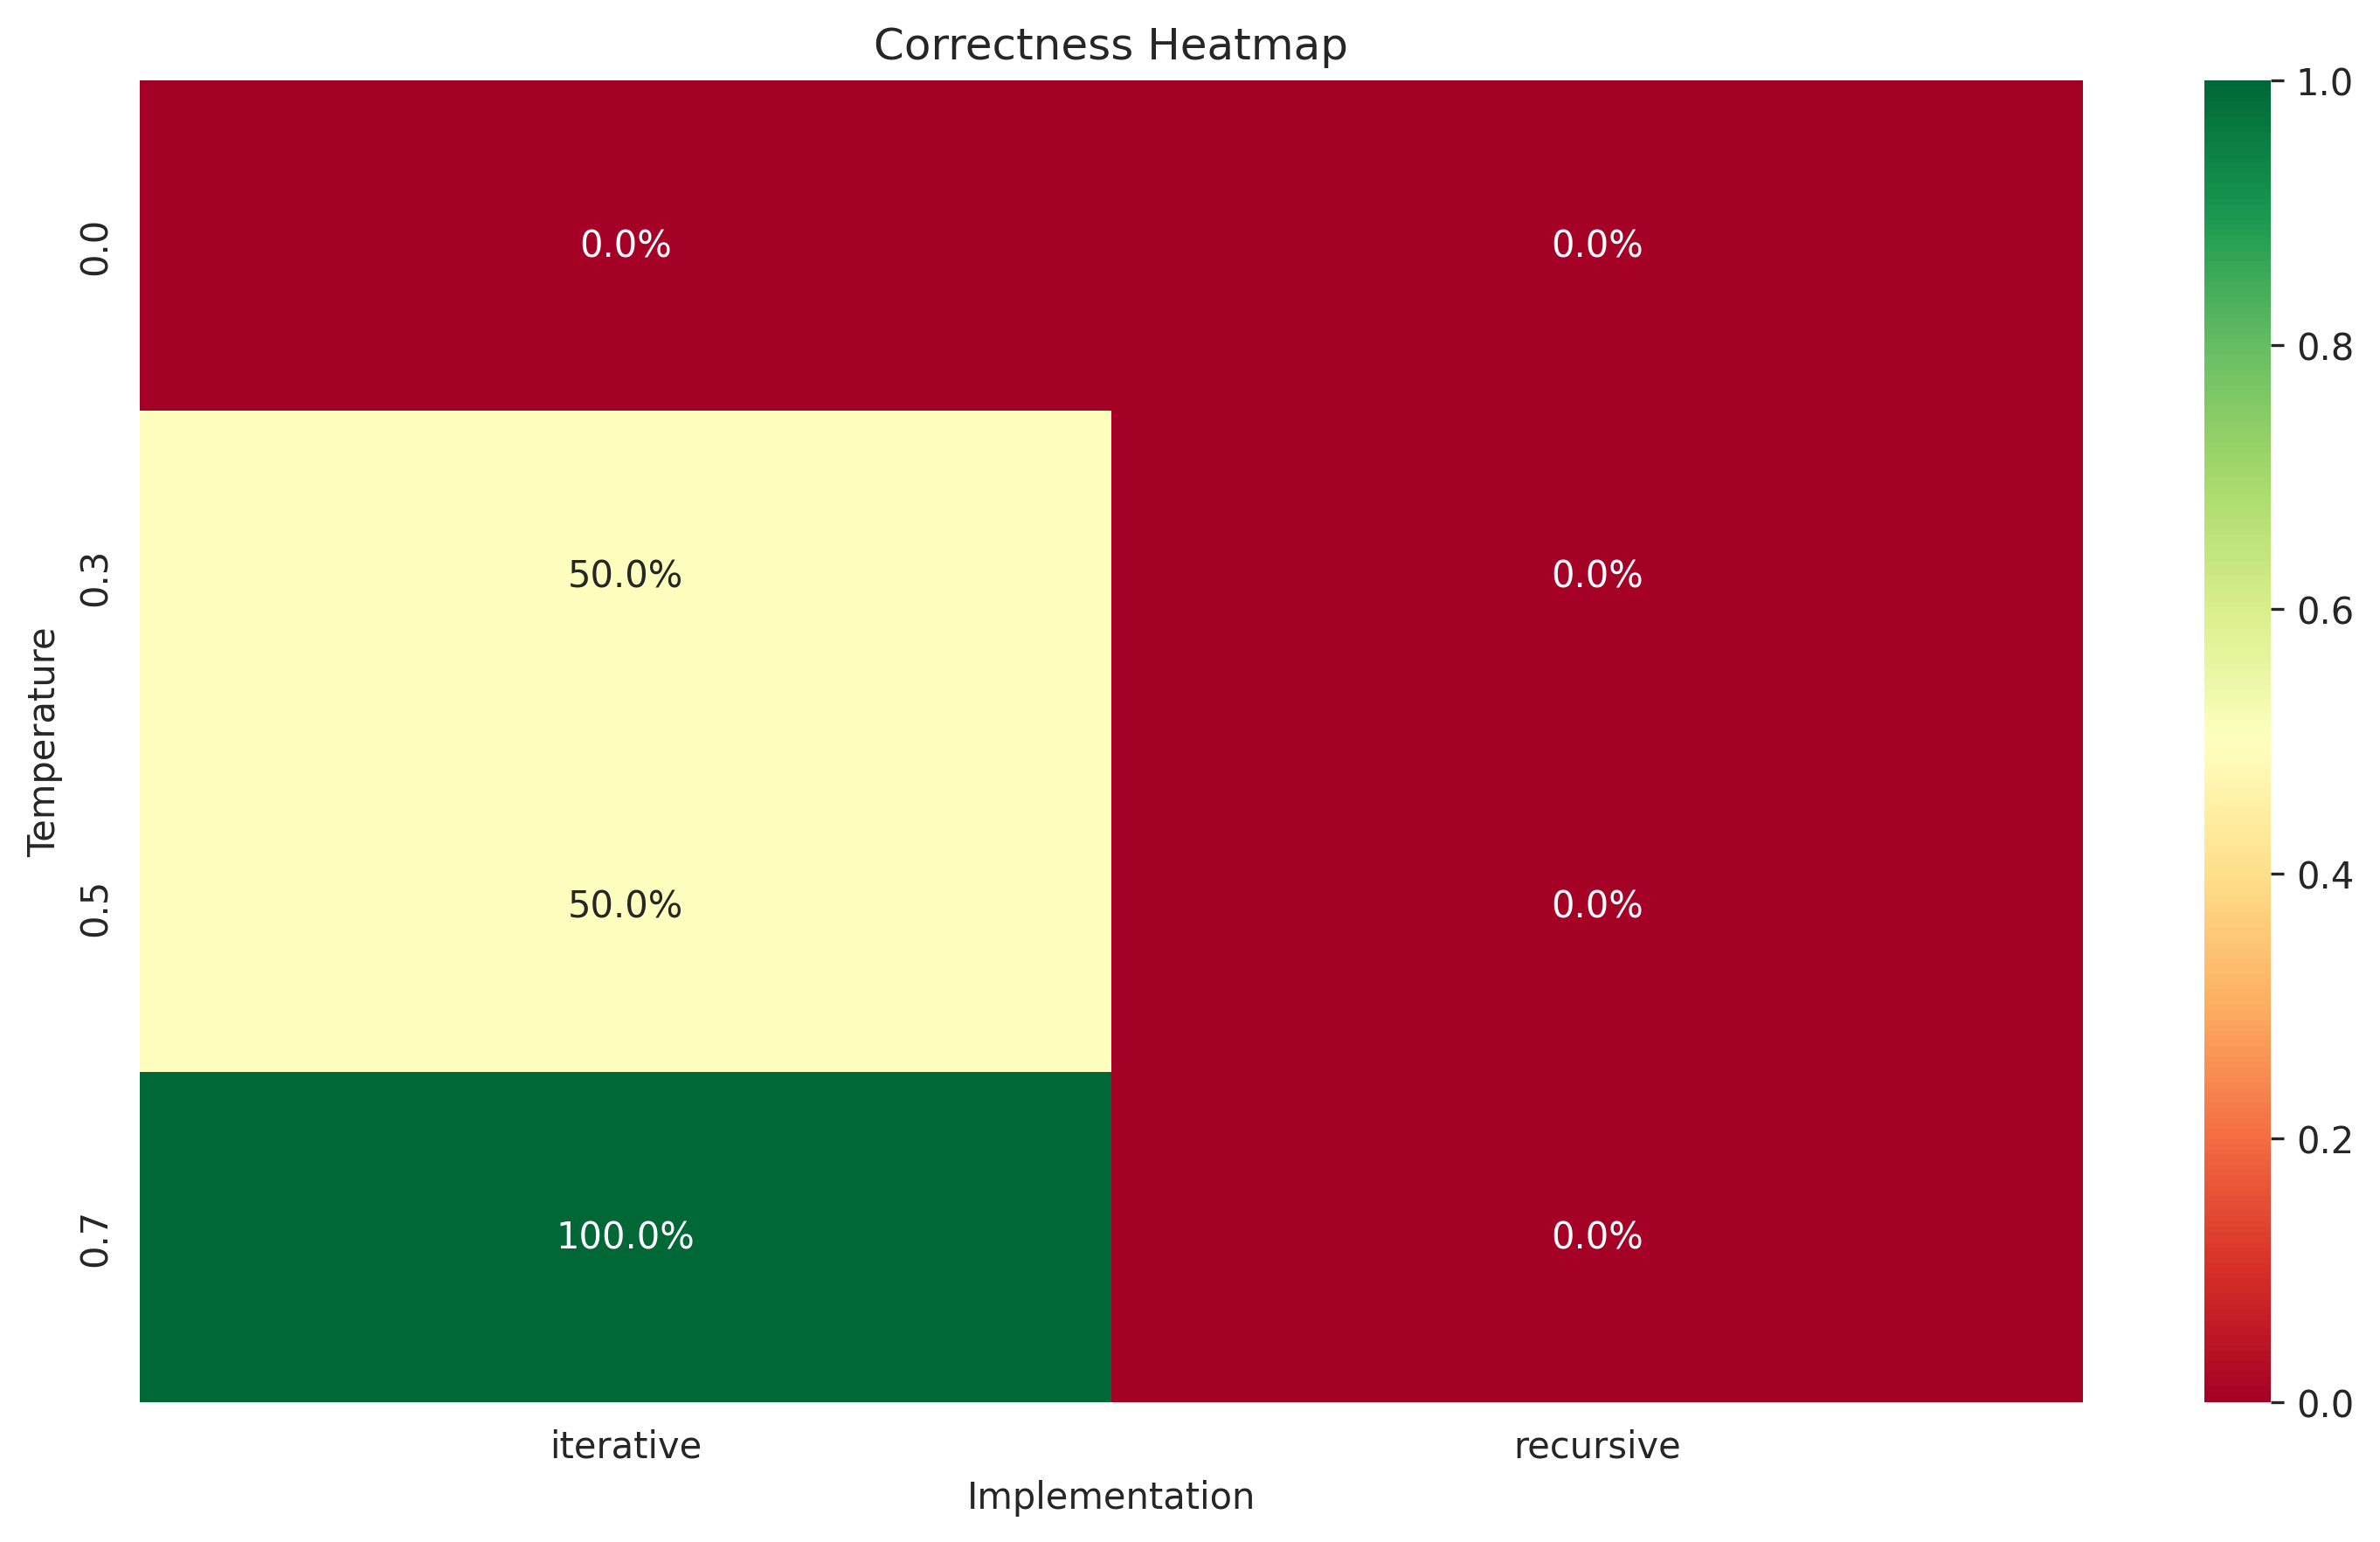
\includegraphics[width=0.65\textwidth]{figures/correctness_heatmap.png}
\caption{Heatmap of correctness rates across temperatures and implementation types.}
\end{figure}

\subsection{Key Observations}

\begin{itemize}
    \item All 16 generated programs were syntactically valid and ran without errors. The model clearly understands Python syntax.
    \item The iterative approach worked well at higher temperatures. At T=0.7, both trials produced correct output.
    \item Greedy decoding (T=0.0) performed worst. The model produced code that ran but gave wrong output for both implementation types.
    \item Recursive implementations failed in all 8 trials. The model understood how to define a recursive Fibonacci function but got the output logic wrong. Instead of printing values while they are less than 100, it typically computed Fibonacci up to index 100 and printed the full list, including large values well above 100.
    \item A small amount of randomness (T=0.7) helped the iterative implementation find the correct solution more reliably.
\end{itemize}

\section{Conclusions}

From these experiments, a few things became clear. First, the model is good at writing code that runs, but getting the logic exactly right is harder, especially for recursive tasks. Second, temperature 0.0 was not the best setting. Some randomness at T=0.7 improved results for iterative code. Third, the iterative approach was more reliable than recursive for this model and task.

The best configuration found was: \textbf{iterative implementation at T=0.7, top-p=0.95}, which produced correct output in both trials.

Overall, the model (0.5B parameters) shows reasonable code generation ability for simple iterative tasks, but struggles with tasks that require reasoning about output filtering in recursive contexts.

\section*{Appendix: Sample Generated Code}

\subsection*{A. Correct Iterative Output (T=0.3)}

\begin{lstlisting}
def fibonacci_sequence():
    a, b = 0, 1
    while a < 100:
        print(a)
        a, b = b, a + b

fibonacci_sequence()
\end{lstlisting}

Output: \texttt{0 1 1 2 3 5 8 13 21 34 55 89} (matches expected output).

\subsection*{B. Incorrect Recursive Output (T=0.7)}

The function logic is correct, but the output filtering is wrong --- it prints a full list up to index 100 instead of stopping when the value exceeds 100.

\begin{lstlisting}
def fibonacci(n):
    if n <= 0:
        return 0
    elif n == 1:
        return 1
    else:
        return fibonacci(n-1) + fibonacci(n-2)

fib_sequence = [0, 1]
for i in range(2, 100):
    fib_sequence.append(fibonacci(i))

print("Fibonacci numbers less than 100:", fib_sequence)
\end{lstlisting}

\begin{thebibliography}{9}

\bibitem{qwen2025coder}
Qwen Team.
\textit{Qwen2.5-Coder Technical Report}.
Alibaba Group, 2024.
Available at: \texttt{https://huggingface.co/Qwen/Qwen2.5-Coder-0.5B-Instruct}

\bibitem{wolf2020transformers}
Thomas Wolf et al.
\textit{Transformers: State-of-the-Art Natural Language Processing}.
Proceedings of EMNLP 2020.

\end{thebibliography}

\end{document}
